\documentclass[MIOP.tex]{subfiles}
\begin{document}

\chapter{Introducción a la Programación\\ Dinámica.}
\section{Introducción.}
La Programación Dinámica (P.D.) son un conjunto de técnicas que permiten resolver procesos de división secuencial.
\begin{ej}
Probabilidad de que al lanzar dos dados sucesivamente tengan antes un suceso que sume 3 a uno que sume 7. Llamemos $A=$``obtener un suceso que sume 3 antes que uno que suma 7''. Tratamos de expresar la probabilidad recursivamente. 

$P(A)=P(A/1er$ lanzamiento suma $3)P(1er$ lanzamiento suma 3$)+P(A/1er$ lanzamiento suma $7)P(1er$ lanzamiento suma $7)+P(A/1er$ lanzamiento no suma ninguno$)P(1er$ lanzamiento no suma ninguno$)$. Sustituyendo por su valor:
$$P(A)=1\cdot\frac{2}{36}+0\cdot\frac{6}{36}+P(A)\frac{28}{36}=\frac{2}{36}+P(A)\frac{28}{36}.$$
Podemos despejar y obtenemos $P(A)=\dfrac{1}{4}$. 
\end{ej}

\begin{ej}
Calcular el factorial de un número recursivamente. Entonces $f(n)=n!=nf(n-1)$. Si sabemos que $f(0)=1$ podemos calcularla para cualquier $n\in\N$.
\end{ej}

\begin{ej}
(Dibujo de Rafa)
Calcular el camino más corto para ir de $1$ hasta $7$. Para llegar al nodo $7$, necesariamente hay que pasar por uno de los $3$ a los que está conectado. Llamamos $l_{ij}$ a la longitud del arco $(i,j)$. Si definimos $f(i)=$``longitud del camino más corto desde $i$ hasta $7$''. Sabemos que $f(7)=0$. 
\[
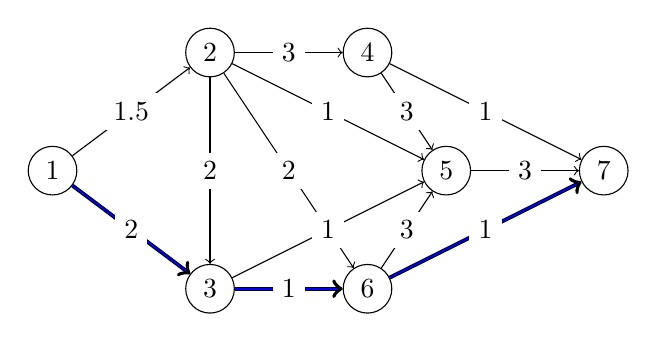
\begin{tikzpicture}
    \node[shape=circle,draw=black] (A) at (0,1.5) {$1$};
    \node[shape=circle,draw=black] (C) at (2,0) {$3$};    
    \node[shape=circle,draw=black] (B) at (2,3) {$2$};
    \node[shape=circle,draw=black] (D) at (4,3) {$4$};
    \node[shape=circle,draw=black] (E) at (4,0) {$6$};
    \node[shape=circle,draw=black] (F) at (5,1.5) {$5$};
    \node[shape=circle,draw=black] (G) at (7,1.5) {$7$};
\tikzset{mystyle/.style={->,double=blue}} 
\tikzset{every node/.style={fill=white}} 
     \path [->] (A) edge node {$1.5$} (B);
     \path [->] (A) edge [mystyle]  node {$2$} (C);
     \path [->] (B) edge node {$2$} (C);
     \path [->] (B) edge node {$1$} (F);
     \path [->] (B) edge node {$2$} (E);
     \path [->] (B) edge node {$3$} (D);
     \path [->] (C) edge [mystyle]  node {$1$} (E);
     \path [->] (C) edge node {$1$} (F);
     \path [->] (D) edge node {$3$} (F);
     \path [->] (D) edge node {$1$} (G);
     \path [->] (E) edge [mystyle] node {$1$} (G);
     \path [->] (F) edge node {$3$} (G);
	 \path [->] (E) edge node {$3$} (F);
\end{tikzpicture}
\]
\begin{align*}
f(4)=&\min\{l_{47},l_{45}+f(5)\}=\min\{1,6\}=1\\
f(5)=&\min\{l_{57}\}=3\\
f(6)=&\min\{l_{67},f(5)+l_{65}\}=\min\{1,3+3\}=1\\
f(3)=&\min\{l_{35}+f(5),l_{36}+f(6)\}=\min\{1+3,1+2\}=3\\
f(2)=&\min\{l_{24}+f(4),l_{25}+f(5),l_{26}+f(6),l_{23}+f(3)\}=\min\{3+1,1+3,2+1,2+2\}=3\\
f(1)=&\min\{l_{12}+f(2),l_{13}+f(3)\}=\min\{1.5+3,2+2\}=4
\end{align*}

Tenemos que el camino más corto tiene longitud $4$ y se corresponde con el camino $1->3->6->7$. Sea $\Gamma(i)=\{j:\exists (i,j)$ en el grafo$\}$. Entonces $f(7)=0$ y $f(i)=\min_{j\in\Gamma(i)}\{l_{ij}+f(j)\}\forall j\neq 7$.

\end{ej}

\subsection{Elementos de P.D.}
\begin{enumerate}
\item El problema se puede descomponer en subproblemas (etapas) y debemos tomar una decisión en cada uno de ellos.
\item En cada etapa hay un número finito de estados.
\item La decisión que se realiza en un estado determina la transición al estado en la etapa siguiente.
\item En un estado, la decisión óptima de los problemas en etapas futuras no depende de las decisiones anteriores. 
\item Debe existir un funcional $f$ que relacióna el valor de un subproblema en la etapa $k$ con el de la etapa $k+1$ (o $k-1$). 
\end{enumerate}

Denotemos por $s_k$ la variable que denota el estado en la etapa $k$. Sea $d_k$ una decisión factible en el estado $s_k$ y $c_k(s_k,d_k)$ el coste incurrido en el estado $k$ si se decide $d_k$. Asimismo, sea $t_k(s_k,d_k)$ el estado al que evoluciona el sistema en la etapa $k+1$ si en $s_k$ se decide $d_k$.

Usando el ejemplo anterior:
\begin{itemize}
\item $s=$nodo.
\item decisiones: $d\in\Gamma(i)$.
\item $c(i,d)=l_{id}$.
\item $t(i,d)=d$.
\end{itemize}

\textbf{Diagrama de cajas}
(dibujo de Rafa)
Etapa $k$:
$\overset{d_k}{\longrightarrow}\boxed{s_k}\rightarrow c_k(s_k,d_k)$\\
Etapa $k$:
$\overset{d_k}{\longrightarrow}\boxed{t_k(s_k,d_k)}\rightarrow c_k(s_{k+1},d_{k+1})$

\begin{defi}
Sea $g:\R^n\to\R$. Decimos que $g$ es \textbf{separable} si $\exists g_1:\R^2\to\R,g_2:\R^{n-1}\to\R$ tales que $g(u_1,u_2,\dots,u_n)=g_1(u_1,g_2(u_2,\dots,u_n))$. 
\end{defi}

\begin{defi}
$g:\R^n\to\R$ es descomponible si
\begin{enumerate}
\item Es separable con $g_1,g_2$ y
\item $g_1$ es monótona no creciente como función de $g_2$ (en proceso de minimización, no decreciente si es maximización). 
\end{enumerate}
\end{defi}

\begin{ej}
Suma, producto de números positivos, máximo... 
\end{ej}

\begin{teorema}[Mitten] 
Sea $g:\R^n\to\R$ una función descomponible con $g_1,g_2$. Asumimos que nos movemos en dominios compactos y las funciones son continuas, de modo que se alcanzan los mínimos. Entonces se verifica:
$$\min_{r_1,r_2,\dots,r_n} g(r_1,r_2,\dots,r_n)=\min_{r_1} g_1(r_1,\min_{r_2,\dots,r_n}g_2(r_2,\dots,r_n))$$

\end{teorema}
\begin{dem}
Dado que $\forall u_1,\dots, u_n$ $g(u_1,\dots, u_n)=g_1(u_1,g_2(u_2,\dots, u_n))$. Entonces $$\min_{r_1,\dots,r_n}g(r_1,\dots,r_n)\leq g_1(u_1,g_2(u_2,\dots, u_n))\forall u_1,u_2,\dots,u_n.$$ Por tanto, $$\min_{r_1,\dots,r_n}g(r_1,\dots,r_n)\leq g_1(u_1,\min_{u_2,\dots,u_n}g_2(u_2,\dots, u_n))\forall u_1.$$ Luego $$\min_{r_1,\dots,r_n}g(r_1,\dots,r_n)\leq \min_{u_1}g_1(u_1,\min_{u_2,\dots,u_n}g_2(u_2,\dots, u_n)).$$
Análogamente, usando que $g_1$ es no creciente en $g_2$, $$g(u_1,\dots, u_n)\geq g_1(u_1,\min_{r_2,\dots,r_n}g_2(r_2,\dots,r_n))\forall u_1.$$ Por consiguiente, 
$$g(u_1,\dots, u_n)\geq \min_{r_1}g_1(r_1,\min_{r_2,\dots,r_n}g_2(r_2,\dots,r_n)).$$ Finalmente,
$$\min_{u_1,\dots,u_n}g(u_1,\dots, u_n)\geq \min_{r_1}g_1(r_1,\min_{r_2,\dots,r_n}g_2(r_2,\dots,r_n)).$$
\end{dem}

\section{Ecuaciones de un proceso de decisión.}
Consideremos un proceso de decisión secuencial en $N$ etapas y denotemos por $s_n$ el estado en la etapa $n$. Supongamos que conocemos el estado final del proceso $s_N^*$. Sean $c_n(s_n,d_n)$ y $t_n(s_n,d_n)$, respectivamente, las funciones de coste entre etapas. Finalmente, supongamos que $f_n(s_n)$ representa el menor coste para ``conducir'' al sistema desde la etapa $n$ en estado $s_n$ hasta $s_N^*$. Entonces, podemos escribir $f_n(s_n)=\min_{d_n}\{c_n(s_n,d_n)+f_{n+1}(t_n(s_n,d_n))\}\ n<N$. Y para $n=N$, $f_N(s_N)=\begin{cases}
+\infty & s_N\neq s_N^*\\
\min_{d_N}c_N(s_N^*, d_N) & s_N=s_N^*
\end{cases}$

Estas ecuaciones se pueden extender a otras funciones $g$ siempre que sean descomponibles.
$f_n(s_n)=\min_{d_n}\{g_1(c_n(s_n,d_n)),f_{n+1}(t_n(s_n,d_n))\}$.
\begin{ejer}[Problema de producción e inventario]
Consideremos un proceso de producción en $T$ etapas, $t=1,2\dots,T$. En la etapa $t$ existe una demanda $d_t$ que hay que satisfacer. En cada etapa se puede decidir producir $x$ unidades  con un coste $c_t(x)$. Además existe un coste de almacén $h_t(I_t)$, que representa el coste en el periodo $t$ por tener $I_t$ unidades al comienzo de este periodo. Suponemos que $I_1=0=I_{T+1}$.  En estado $I_t$, $f_t(I_t)$ es el mínimo coste para atender la demanda desde $t$ a $T$ si en $t$ tengo $I_t$ en inventario. Entonces $f_t(I_t)=\min_{x}\{c_t(x)+f_{t+1}(I_t+x-d_t)\}$ si $t<T+1$ y $f_{T+1}=\begin{cases}
+\infty & I_{T+1}>0\\
0 & I_{T+1}=0
\end{cases}$

La solución del problema es $f_1(0)$. Resolver el problema con los siguientes datos.

\begin{tabular}{|c| c c c c|}
\hline
$t$ & $1$ & $2$ & $3$ & $4$\\
\hline
$d_t$ & $1$ & $3$ & $2$ & $4$\\
\hline

\end{tabular}

$I_1=I_5=0$, $h_t(I)=\frac{1}{2}I$ ($I\leq 4$), $c_t(x)=\begin{cases}
3+x & 5\geq x>0\\
0 & x=0
\end{cases}$
\end{ejer}

\end{document}
